\documentclass[12pt]{article}
\usepackage[utf8]{inputenc}
\usepackage{latexsym,amsfonts,amssymb,amsthm,amsmath}
\usepackage[T1, T2A]{fontenc}% T2A for Cyrillic font encoding
\usepackage[bulgarian]{babel}
\usepackage{float}
\usepackage{graphicx}
\usepackage{amssymb}
% \usepackage{emoji}
\usepackage{hyperref}
\usepackage[
backend=biber,
style=alphabetic,
]{biblatex}
\newcommand{\cyrchar}[1]{\foreignlanguage{bulgarian}{#1}}


\graphicspath{ {./images/} }


\setlength{\parindent}{0in}
\setlength{\oddsidemargin}{0in}
\setlength{\textwidth}{6.5in}
\setlength{\textheight}{8.8in}
\setlength{\topmargin}{0in}
\setlength{\headheight}{18pt}

\begin{document}
	
	\title{ Подходи за обработка на естествен език \newline SemEval-2025 Task-3 — Mu-SHROOM  \newline}
	
	
	\author{Кристиян Симов, ф.н. 4MI3400288 \\ Цветан Цветанов, ф.н. 4MI3400570 \\ Изкуствен интелект}
	\maketitle
	
	% \begin{Logo}
		\begin{figure}[H]
			\centering
			
\includegraphics[width=0.25\linewidth]{clement-ohrid-logo.png}
		\end{figure}
		
		\begin{figure}[H]
			\centering
			
\includegraphics[width=0.25\linewidth]{fmi-logo.jpg}
		\end{figure}
		% \end{Logo}
	
	
	\vspace{0.5in}
	\pagebreak
	
	\section{Въведение}
	
	Големите езиковите модели владеят естествените езици и звучат убедително. Но понякога генерират грешни и подвеждащи твърдения,  които нямат връзка със заявката на потребителя  или реална подкрепа с факти.  От друга страна, съществуващите метрики са пригодени по-скоро да  описват  нивото на владеене на езика от модела, отколкото неговата коректност. \newline
	
	Халюцинирането е един от ключовите все още неразрешени проблеми  на големите езикови модели.  Задачата  Mu-SHROOM в изданието на SemEval от 2025 е продължение на SHROOM от миналогодишното издание. През 2024 година задачата пред участниците е била да класифицират дали даден текст е халюцинация (да или не). Промяната в сегашното издание е, че се очаква да се предскаже началото и края на халюцинация в изходния текст на конкретен модел.
	
	\section{Данни}
	
	Използвани са единствено публично достъпните данни от \href{https://helsinki-nlp.github.io/shroom/}{страницата на задачата}. Не е правен опит да се генерират синтетични данни. Организаторите са подготвили текстови данни за трениране, тестване и валидация на 14 различни езика -  арабски (модерен стандартен), баски, каталонски, китайски (мандарин), чешки, английски, фарси, финландски, френски, немски, хинди, италиански, испански и шведски. Данните са предоставени в jsonl формат. Всеки ред от тези файлове отговаря на json обект:
	
	\begin{figure}[H]
		\centering
		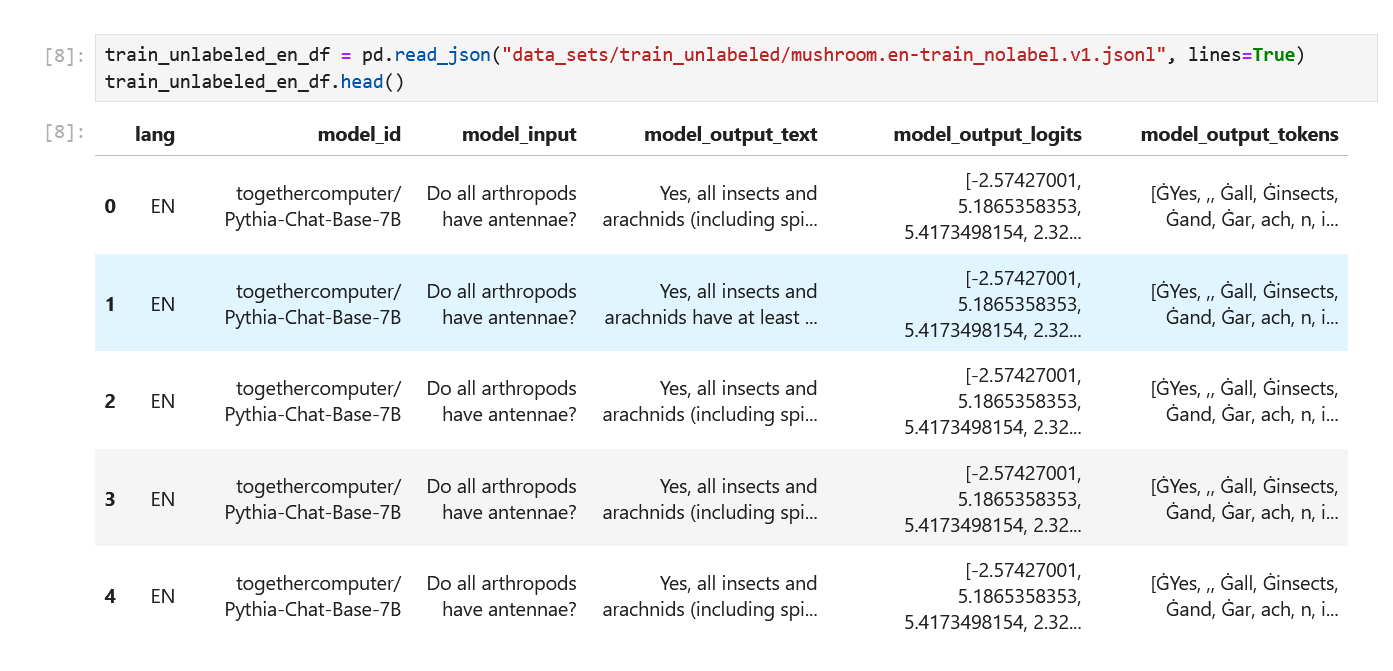
\includegraphics[width=1\linewidth]{trainset.png}
		\caption{Английско обучаващо множество}
	\end{figure}
	%	Данните за всеки език 
	
	
	
	\section{Метод}
	
	\subsection{Обработка на данните}
	
		\begin{enumerate}    
			\item[\textbullet] Токенизиране  изхода на модела - с цел генериране речник на отместванията (offset mapping)
			\item[\textbullet] Векторизиране входа на потребителя и изходните токени
			\item[\textbullet] Чистене на аномалии чрез регулярен израз - технически токени в изходните токени и съответните им логити
			\end{enumerate}
	
	\subsection{Алгоритми} 
	
	Използвана е невронна мрежа със стохастично градиентно спускане (Adam optimizer) за изчисление на вероятност за потискане на токен базирайки се на логити и на семантична близост. Хиперпараметри на оптимизатора са: наказателен параметър (за да ограничи склонността към потискане), параметър на ентропията (насърчава вероятностите за потискане да са близо до 0 или 1), скорост на обучение и брой епохи.
	
	Алгоритъмът на обучение използва крос-ентропия като функция на загубата между вероятностното разпределение на вгражданията на входа и съответното разпределение на вгражданията на  маскираните изходи. 
	Голямата цел на тези сложни сметки и трансформации е да определим в кой конкретен токен започва халюцинацията.
	\section{Експерименти}
	
	\begin{enumerate}    
		\item[\textbullet] Опити с  различни стойности на хиперпараметрите и сравнение на резултатите с цел опитмизация
		\item[\textbullet] Експерименти с Vectara Hallucination model приложена към двойки от входни заявки и изходни токени
		\item[\textbullet] Чистене на аномалии чрез регулярен израз - технически токени в изходните токени и съответните им логити
	    \item[\textbullet] Евристики за разпръскване на определено количество вероятностна маса над определен праг в съседни вероятности (с цел "заразяване" на съседни токени).
	     \item[\textbullet] Обучаване на модела с различни подмножества от обучаващите множества езици
	     \item[\textbullet] Генериране диапазони на халюцинация със и без речници на отстъпа
	\end{enumerate}
	
	\section{Резултати}
	
	\href{https://github.com/Kr1s1m/SemEval-2025_Task-3/}{Публично Github хранилище с кода от проекта} 
	\href{https://mushroomeval.pythonanywhere.com/submission/}{Официално класиране}
	
	\section{Заключение и бъдеща работа}
	
	Както се вижда от предната секция, модел o1\_toy постига най-добра точност за английски ($\approx$ 17\% IoU \textnumero 39), немски ($\approx$ 13\% IoU \textnumero 28), арабски ($\approx$ 11\% IoU, \textnumero 29). Тези по-добри резултати в сравнение с останалите езици се дължат на наличието отворени токенизатори за съответните езикови модели, с които могат да се генерират речници за отстъпа. За сравнение без речници: английски ($\approx$ 13\% IoU), немски ($\approx$ 10\% IoU) арабски ($\approx$ 7\% IoU). Корелацията на Спиърман (Cor) между генерираните от модела вероятности, назначавани на всеки предсказан диапазон съдържащ халюцинации, и вероятностите от златните корпуси като цяло е ниска и дори отрицателна.
	\newline\newline Идеи за бъдещо подобрение:
	
	\begin{enumerate}    
		\item[\textbullet] Генериране на речници за отстъпа (offset mappings) за всички езици
		\item[\textbullet] Vectara за вграждания и вероятност за халюцинация
		\item[\textbullet] RAG за проверка на фактологията
		\item[\textbullet] Смяна BERT модела за по-подходящи вграждания
		\item[\textbullet] По-фино оптимизиране хиперпараметрите
		\item[\textbullet] Съкращаване времето за обучение на невронната мрежа
		\item[\textbullet] Изчисляване с точни метрики представянето на нашия модел - f1, precision, recall.

	\end{enumerate}

	\section{Индивидуален принос}
	
	Нашият екип вярва в гъвкавите принципи на разработка като  \href{https://asana.com/resources/extreme-programming-xp}{extreme programming(XP)} и по конкретно pair programming. Поради ограниченото време, с което разполагаше екипът преди крайния срок за участие в SemEval, много голяма част от проучването, разработката, експериментите и писането на документация беше споделена във виртуална среда. Това улесни комуникацията и синхронизацията, освен това доведе до бързо тестване на прототипи и ранно откриване на грешки.
	
\end{document}